\chapter{Diseño y Arquitectura}
\section{Arquitectura MVT de Django}
El sistema está construido siguiendo el patrón Modelo-Vista-Template (MVT) de Django, que separa la lógica de negocio, la presentación y el acceso a datos \cite{django-docs}. Esta arquitectura facilita la mantenibilidad, escalabilidad y reutilización de componentes. El modelo representa la estructura y reglas de los datos, la vista gestiona la lógica de negocio y las respuestas a las solicitudes del usuario, y el template define la presentación visual de la información.

\begin{figure}[H]
	\centering
	% Diagrama UML de la arquitectura general (PlantUML)
	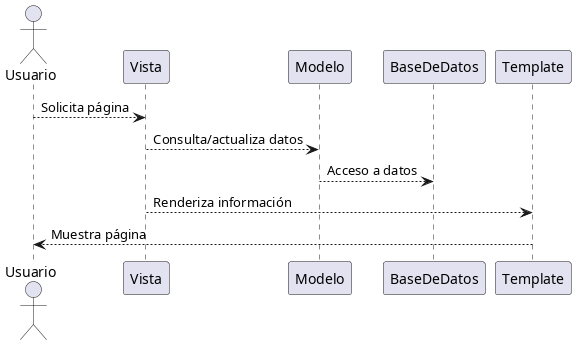
\includegraphics[width=0.8\textwidth]{uml/arquitectura-mvt.png}
	\caption{Diagrama UML de la arquitectura MVT de Django para el sitio LIESE.}
\end{figure}
\newpage
\section{Modelos de Datos}
El modelo de datos del sitio LIESE incluye entidades como Miembro, Proyecto, Artículo, Evento, Noticia y Solicitud de Oportunidad. Cada entidad se implementa como una clase en Django, con atributos que representan los campos de la base de datos y relaciones entre modelos (por ejemplo, un artículo tiene un autor que es un miembro, y un proyecto puede tener varios miembros asociados). El uso del ORM de Django permite definir, consultar y migrar los modelos de manera eficiente y segura.

\begin{figure}[H]
	\centering
	% Diagrama UML de clases de los modelos principales (PlantUML)
	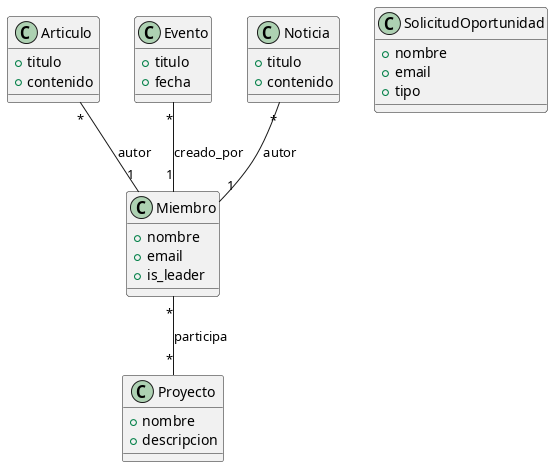
\includegraphics[width=0.95\textwidth]{uml/modelos-datos.png}
	\caption{Diagrama UML de clases de los modelos principales del sistema LIESE.}
\end{figure}
\newpage
\section{Diseño de Base de Datos}
La base de datos se diseña para soportar la gestión de información académica y administrativa del laboratorio. Se emplea SQLite en desarrollo y PostgreSQL en producción, aprovechando la portabilidad y robustez de ambos motores \cite{postgresql-docs}. Las migraciones de Django permiten evolucionar el esquema de datos sin pérdida de información. El diseño contempla claves foráneas para mantener la integridad referencial y relaciones muchos a muchos (por ejemplo, miembros y proyectos).

\begin{figure}[H]
	\centering
	% Diagrama UML entidad-relación simplificado (PlantUML)
	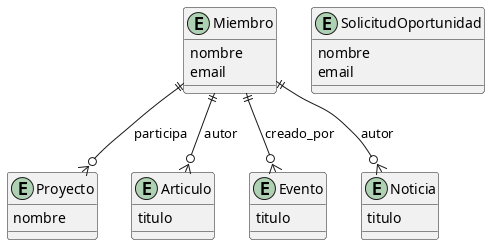
\includegraphics[width=0.95\textwidth]{uml/diagrama-er.png}
	\caption{Diagrama entidad-relación (ER) simplificado de la base de datos.}
\end{figure}
\section{Arquitectura de Templates}
La presentación del sitio se implementa mediante el sistema de templates de Django, que permite separar la lógica de presentación del código Python. Se utilizan plantillas HTML con etiquetas y filtros de Django para renderizar información dinámica, y se heredan estructuras comunes como la barra de navegación y el pie de página. El uso de Bootstrap facilita el diseño responsivo y accesible \cite{bootstrap-docs}.

\begin{figure}[H]
	\centering
	% Diagrama UML de herencia de templates (PlantUML)
	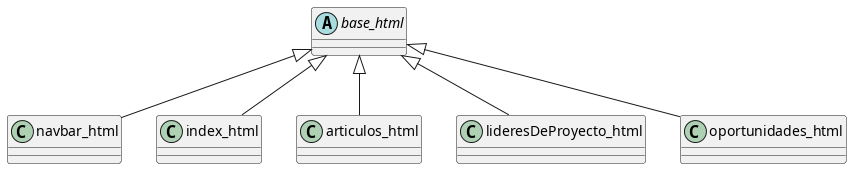
\includegraphics[width=0.7\textwidth]{uml/templates-herencia.png}
	\caption{Diagrama de herencia de templates en el sistema LIESE.}
\end{figure}
